Disinfection booster stations are commonly used throughout water distribution networks 
to maintain drinking water standards. Disinfectants degrade as they move through the 
system and booster stations, designed to inject disinfectant at strategic locations, 
help maintain residual levels. Booster stations can also be placed with 
water security objectives in mind. WST includes two booster subcommands, \code{booster\_msx} 
and \code{booster\_mip} that are 
designed to place booster stations to minimize the impact of a contamination incident. 
These subcommands use different approaches to model the reaction dynamics between 
a contaminant and disinfectant. 

The \code{booster\_msx} subcommand uses EPANET-MSX to 
simulate the reaction dynamics between the contaminant and disinfectant. 
A flowchart representation of the \code{booster\_msx} subcommand is shown 
in Figure \ref{fig:booster_msx_flowchart}. The \code{booster\_msx} subcommand employs 
an iterative process that combines contaminant transport, impact assessment 
and optimization. The optimization process identifies a set of booster station locations 
where disinfectant is injected. The contaminant and disinfectant injections and their 
reaction dynamics are simulated in the contaminant transport 
process and the effectiveness of the booster injections are evaluated based upon 
the impact assessment process. Since the \code{booster\_msx} subcommand relies 
on the \code{tevasim} and \code{sim2Impact} subcommands, their required input 
is also required for the \code{booster\_msx} subcommand. Additionally, the sensor network 
design used to detect the contamination incident(s) and the booster station characteristics 
are required inputs. The utility network model is defined by a EPANET 2.00.12 INP file, 
while the rest of the input can be specified in the \code{booster\_msx} WST configuration file.

\begin{figure}[h]
  \centering
  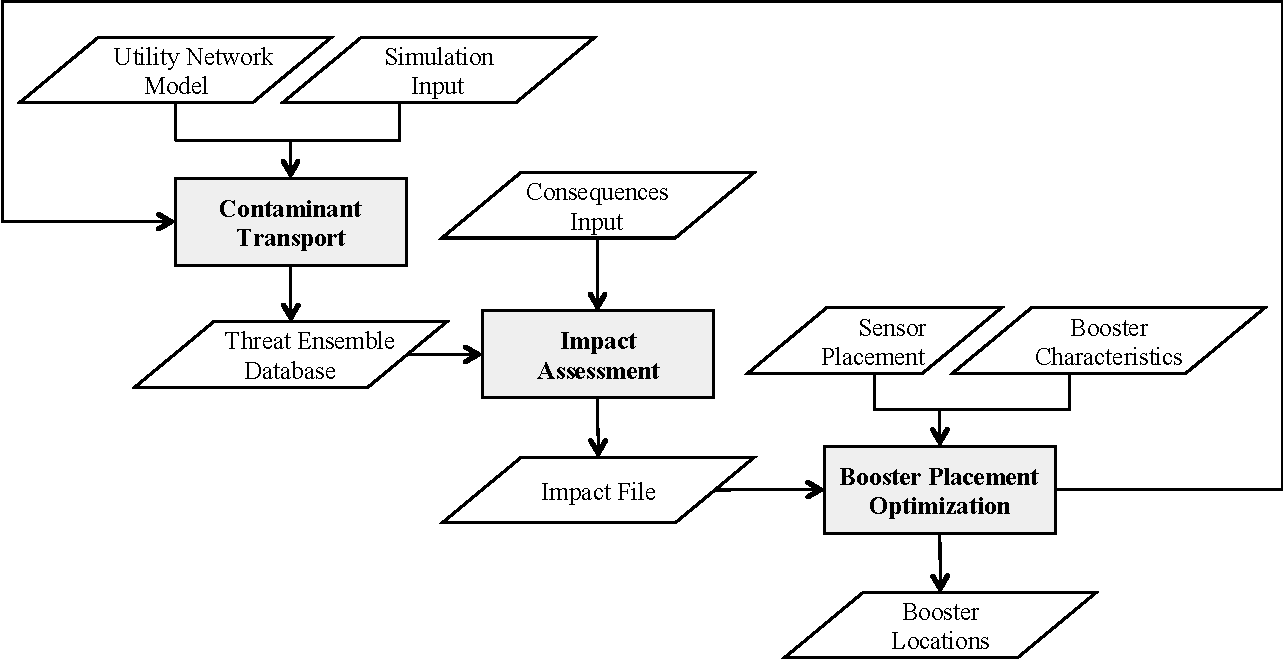
\includegraphics[scale=0.75]{graphics/booster_msx_flowchart.pdf}
  \caption{Multi-species reaction booster placement flowchart.}
  \label{fig:booster_msx_flowchart}
\end{figure}

The \code{booster\_mip} 
subcommand uses the linear water quality model Merlion and assumes the reaction dynamics between the contaminant and 
disinfectant can be approximated by a neutralization or limiting reagent reaction model.
A flowchart representation of the \code{booster\_mip} subcommand is shown in Figure \ref{fig:booster_mip_flowchart}. 
The utility network model is defined by a EPANET 2.00.12 INP file. Additional input specified in the \code{booster\_mip} WST 
configuration file are the contamination scenarios, the sensor network design used to detect 
the contamination incident(s) and the booster station characteristics. 

\begin{figure}[h]
  \centering
  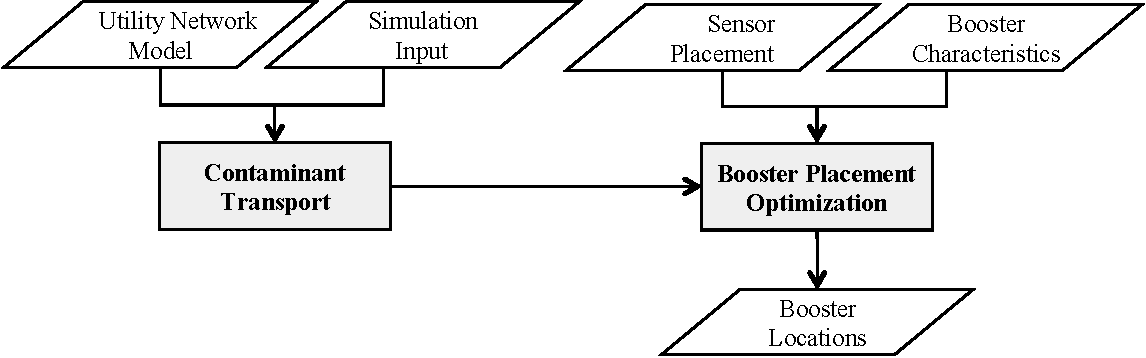
\includegraphics[scale=0.75]{graphics/booster_mip_flowchart.pdf}
  \caption{MIP booster placement flowchart.}
  \label{fig:booster_mip_flowchart}
\end{figure}

\section{Booster Placement Using Multi-species Reaction}\label{booster_msx_formulations}

The \code{booster\_msx} subcommand uses optimization methods integrated 
with EPANET-MSX to evaluate booster placements using multi-species reaction dynamics between 
the contaminant and disinfectant. The booster station placement problem formulation 
selects a set of booster station locations that minimizes the average impact 
of all contamination incidents given a set of potential booster stations that 
inject a disinfecting agent. The mathematical formulation can be written as follows:
\begin{align}
\textrm{  minimize } \qquad & \dfrac{1}{A} \sum_{a \in {A}}d_{a,\max} \label{eqn:booster_msx} \\
\textrm{subject~to } \qquad &\sum_{b\in B}y_{b} \leq B_{\max} \label{eq:booster_msx_2} \\
&y_{b} \in \{0,1\} &&\forall b\in B \label{eq:booster_msx_3}
\end{align}
where ${A}$ represents a set of contamination incidents, 
$d_{a,\max}$ defines the maximum impact of the contamination incident $a$, 
$B$ represents the set of potential booster station locations,
$y_b$ is a binary variable which is 1 if node $b$ is selected as a booster station location 
and $B_{\max}$ is the maximum number of booster station locations. 
The maximum impact of a contamination incident, $d_{a,\max}$, is the total impact 
across the entire network at the end of the simulation assuming that the 
contaminant was not detected by a sensor, and no interventions to reduce 
impacts were implemented. This value is found in the -1 entry of the impact file. 
For this problem, it is assumed that booster stations can be located at any 
user-defined nodes in the network.

\subsection{Booster MSX Solvers}
The multi-species booster station placement problem is solved through an iterative optimization process which 
selects different sets of booster station locations and evaluates their effectiveness
in minimizing the impact of a set of contamination incidents. Two optimization 
methods, an evolutionary algorithm and a network solver, are available in WST to solve this problem. 
Each solver is explained in more detail in the following subsections. 

\subsubsection{Evolutionary Algorithm}\label{boostermsx_coliny_ea}
The evolutionary algorithm (EA) included with DAKOTA, Coliny EA, is used in the 
optimization routine for the \code{booster\_msx} subcommand. 
Additional information on DAKOTA/Coliny solvers can be found at 
\url{http://dakota.sandia.gov/docs/dakota/5.2/html-ref/index.html}
and in the DAKOTA user manual \citep{DakotaUserManual}.
The random number generator used in Coliny EA is platform dependent.  
This can result in slight variations in the solution.

To design an EA, the parameter space for the optimization problem is first 
encoded into a string of numbers. This encoded representation of the problem 
is called a genetic string, where each element of the genetic string represents 
one parameter. When the EA is used with \code{booster\_msx}\, the parameter space 
is defined by the number of booster station locations. Each location is assigned a sequential 
integer that represents a feasible location within the EPANET network. The final EA solution is 
translated to represent EPANET node IDs.

The EA has several solver options that define how the EA evolves. These options can be set in the 
\code{[solver][options]} sections of the \code{booster\_msx} WST configuration file and are specific to the Coliny EA solver. 
The EA evolves an initial genetic strings of size \code{[population\_size]} that is 
set based on \code{[initialization\_type]} using the following steps:
\begin{enumerate}
\item Evaluation: Evaluate the solution for each genetic string. This involves function 
calls to the \code{tevasim} and \code{sim2Impact} subcommands for each string to define the fitness score.  
\item Breeding: Select two members of the population based on fitness. The 
probability of selection is based on \code{[fitness\_type]}.  
\item Crossover: Crossover two members based on \code{[crossover\_type]} and \code{[crossover\_rate]}. 
\item Mutation: Mutate the two members based on \code{[mutation\_type]} and \code{[mutation\_rate]}.
\item Steps 2-4 are repeated until the entire population has been changed.
\item Replacement: After a new population is created, the old population is 
replaced by the current population while keeping the highest ranked string 
(elitist = 1 replacement option).
\end{enumerate}
Steps 1-6 are repeated until \code{[max\_iterations]} or \code{[max\_function\_evaluations]} criteria is met. 

\subsubsection{Network Solver}\label{boostermsx_coliny_statemachine}

The network solver used in WST is a network-constrained, derivative-free local search optimization algorithm. 
It is a discrete analog-to-pattern search. The allowable moves are to adjacent nodes, rather than moves in the 
continuous space. This approach provides local refinement of candidate solutions. The valid moves include
removing a node location and replacing it with one anywhere in the network. Two forms of the network solver can be 
used: with and without initial starting points. The initial starting points are node locations in the network
in which the algorithm should begin its local search. If these points are not supplied to the algorithm, 
then it reduces to a greedy placement algorithm. Convergence is met when no remaining moves improve the solution.

\if 0
\subsubsection{Parallelization}

The Dakota coliny\_ea and StateMachineLS solvers both include an option to set 
the number of threads used to perform the simulations.   
This option is specified in \code{[solver][threads]}, as shown below. It should be 
set to the number of threads that are available for the simulation. The default value is 1.  
If an integer greater than 1 is specified, Dakota will run that many threads.
The expected efficiency of parallelization is nearly linear with the number of 
threads (up to the number of processor cores in the computer).

\begin{unknownListing}
solver:
  type: coliny_ea 
  threads: 2
\end{unknownListing}

\subsubsection{Stop time criteria}

If a solution needs to be identified within a certain amount of time, a simulation stop time 
criteria can be defined. This option causes the solver to terminate after a 
specified time, even if the underlying algorithm has not converged to an optimal solution.  
The stop time criteria is included with both the Dakota coliny\_ea and 
StateMachineLS solvers, and it is specified in \code{[solver][options][misc\_options]}, as 
shown below. The max\_time has to be given in seconds. As the optimization 
algorithms only check the elapsed time once per major iteration, the actual 
solver run time will be slightly longer than the specified maximum run time.  
When the optimization process is cut off prematurely, the best solution 
obtained so far is reported to the user.

\begin{unknownListing}
solver:
  type: StateMachineLS  
  options: 
    misc_options: "'max_time=10'"
\end{unknownListing}

% \subsubsection{Skeletonization}

% To reduce the size of the network model, possible contamination incidents and the number of 
% feasible booster station locations, the user can skeletonize the problem and evaluate 
% the results on the full network model. WST includes a utility script, spotSkeleton,  
% that can be used to skeletonize network models (See Executable Files Section ~\ref{skelExecutable}).  
% Network models are skeletonized based on a pipe diameter threshold. The executable, spotSkeleton,  
% creates a new EPANET input (inp) file and a related map file.  
% The map file associates the nodes in the skeletonized network model (upscaled nodes)  
% to the nodes in the original network model (downscaled nodes). When  
% working with a skeletonized network model, other aspects of the booster station problem also  
% need to upscaled based on the skeletonization map. These include: the injection location(s)  
% and strength of the contamination incident(s), the population at each node, the sensor  
% placement, the feasible booster station locations, and the initial points for the optimization  
% solver. For example, if Nodes 1, 2, 3 and 4 in the original network model are  
% represented by Node 2 in the skeletonized network model, then a sensor placed at  
% Node 4 in the original network model should be placed at Node 2 in the skeletonized  
% network model. 

% After booster station optimization is run on the skeletonized network model, the  
% solution can then be evaluated or refined using the original network model.  
% To evaluate the current solution, the locations on the skeletonized network 
% should be listed as the only feasible booster station locations  
% in the original network model and the EVALUATE solver option should be used (See Example ~\ref{booster_ex2}}).   
% To refine the current solution, downscale the locations on the skeletonized network
% and use those original network nodes as the only feasible booster station locations  
% in a second optimization. In this refinment, the solver type and  
% solver options can be different for the first and second optimization.
\fi

\subsection{\code{booster\_msx} Subcommand}

The \code{booster\_msx} subcommand is executed using the following command line:
\begin{unknownListing}
wst booster_msx <configfile> 
\end{unknownListing}
where \code{configfile} is a WST configuration file in the YAML format. 

The \code{---help} option prints information about this subcommand, such as usage,
arguments and a brief description:
\begin{unknownListing}
wst booster_msx --help
\end{unknownListing}

\subsubsection{Configuration File}

The \code{booster\_msx} subcommand generates a template configuration file using the following command line:

\begin{unknownListing}
wst booster_msx --template <configfile>
\end{unknownListing}

The \code{booster\_msx} template configuration file is shown in Figure \ref{fig:booster_msx_template}.  
Brief descriptions of the options are included in the template after the \# sign.  

\begin{figure}[p!]
  \unknownInputListing{examples/booster_msx_config.yml}{}{1}{47}
  \caption{The \code{booster\_msx} configuration template file.}
  \label{fig:booster_msx_template}
\end{figure}

\subsubsection{Configuration Options}

Full descriptions of the WST configuration options used by the \code{booster\_msx} subcommand are listed below.
\begin{description}[topsep=0pt,parsep=0.5em,itemsep=-0.4em]
  \item[{network}]\hfill
  \begin{description}[topsep=0pt,parsep=0.5em,itemsep=-0.4em]
    \item[{epanet file}]\hfill
\\ The name of the EPANET 2.00.12 input (INP) file that defines the water distribution
                network model.
                
                Required input.
  \end{description}
  \item[{scenario}]\hfill
  \begin{description}[topsep=0pt,parsep=0.5em,itemsep=-0.4em]
    \item[{location}]\hfill
\\A list that describes the injection locations for the contamination scenarios.
                The options are: (1) ALL, which denotes all nodes (excluding tanks and reservoirs)
                as contamination injection locations; (2) NZD, which denotes all nodes with
                non-zero demands as contamination injection locations; or (3) an EPANET node ID, 
                which identifies a node as the contamination injection location. This allows 
                for an easy specification of single or multiple contamination scenarios.
                
                Required input unless a TSG or TSI file is specified.
    \item[{type}]\hfill
\\The injection type for the contamination scenarios. The options are MASS, CONCEN, FLOWPACED or SETPOINT. 
                See the EPANET 2.00.12 user manual for additional information about source types \citep{EPANETusermanual}.
                
                Required input unless a TSG or TSI file is specified.
    \item[{strength}]\hfill
\\The amount of contaminant injected into the network for the contamination scenarios.  
                If the type option is MASS, then the units for the strength are in mg/min. 
                If the type option is CONCEN, FLOWPACED or SETPOINT, then units are in mg/L.
                
                Required input unless a TSG or TSI file is specified.
    \item[{species}]\hfill
\\The name of the contaminant species injected into the network. This is the name of a single species. 
                It is required when using EPANET-MSX, since multiple species might be simulated, but
                only one is injected into the network. For cases where multiple contaminants are injected,
                a TSI file must be used.
                
                Required input for EPANET-MSX unless a TSG or TSI file is specified.
    \item[{start time}]\hfill
\\The injection start time that defines when the contaminant injection begins. 
                The time is given in minutes and is measured from the start of the simulation. 
                For example, a value of 60 represents an injection that starts at hour 1 of the simulation.
                
                Required input unless a TSG or TSI file is specified.
    \item[{end time}]\hfill
\\The injection end time that defines when the contaminant injection stops.				
                The time is given in minutes and is measured from the start of the simulation.
                For example, a value of 120 represents an injection that ends at hour 2 of the simulation.
                
                Required input unless a TSG or TSI file is specified.
    \item[{tsg file}]\hfill
\\The name of the TSG scenario file that defines the ensemble of contamination
                scenarios to be simulated. Specifying a TSG file will
                override the location, type, strength, species, start and end times options specified in
                the WST configuration file. The TSG file format is documented in File Formats Section \ref{formats_tsgFile}.
                
                Optional input.
    \item[{tsi file}]\hfill
\\The name of the TSI scenario file that defines the ensemble of contamination
                scenarios to be simulated. Specifying a TSI file will
                override the TSG file, as well as the location, type, strength, species, start and end time options specified in
                the WST configuration file. The TSI file format is documented in File Formats Section \ref{formats_tsiFile}.
                
                Optional input.
    \item[{signals}]\hfill
\\Name of file or directory with information to generate 
                or load signals. If a file is provided the list of inp tsg tuples
                 will be simulated and the information stored in signals files. If
                a directory with the signals files is specified, the signal files will
                be read and loaded in memory. This input is only valid for the uq
                subcommand and the grabsample subcommand with probability based formulations.

                Optional input.
    \item[{msx file}]\hfill
\\The name of the EPANET-MSX multi-species file that defines the multi-species reactions to
                be simulated using EPANET-MSX.
                
                Required input for EPANET-MSX.
    \item[{msx species}]\hfill
\\The name of the MSX species whose concentration profile will be saved by the EPANET-MSX simulation
                and used for later calculations.
                
                Required input for EPANET-MSX.
    \item[{merlion}]\hfill
\\A flag to indicate if the Merlion water quality
                simulator should be used. The options are true or false. 
                If an MSX file is provided, EPANET-MSX will be used.
                
                Required input, default = false.
  \end{description}
  \item[{impact}]\hfill
  \begin{description}[topsep=0pt,parsep=0.5em,itemsep=-0.4em]
    \item[{erd file}]\hfill
\\The name of the ERD database file that contains the 
                contaminant transport simulation results. It is 
                created by running the \code{tevasim} subcommand.
                Multiple ERD files (entered as a list, i.e., [<file1>, <file2>]) can be combined to
                generate a single impact file. This can be used to combine
                simulation results from different types of contaminants, in
                which the ERD files were generated from different
                TSG files.
                
                Required input.
    \item[{metric}]\hfill
\\The impact metric used to compute the impact file. Options
                include EC, MC, NFD, PD, PE, PK, TD or VC. One impact file 
                is created for each metric selected. These metrics are 
                defined in Section \ref{impact_measures}.
                
                Required input.
    \item[{tai file}]\hfill
\\The name of the TAI file that contains health impact information. 
                The TAI file format is documented in File Formats Section \ref{formats_taiFile}.
                
                Required input if a public health metric is used (PD, PE or PK).
    \item[{response time}]\hfill
\\The number of minutes that are needed to respond to the
                detection of a contaminant. This represents the time that it takes
                a water utility to stop the spread of the contaminant in the network and 
                eliminate the consumption of contaminated water. As the response time increases,
                the impact increases because the contaminant affects the network
                for a greater length of time.  
                
                Required input, default = 0 minutes.
    \item[{detection limit}]\hfill
\\The minimum concentration that must be exceeded before a sensor can detect a contaminant.
                There must be one threshold for each ERD file. The units of
                these detection limits depend on the units of the contaminant
                simulated for each ERD file (e.g., number of cells of a
                biological agent).  
                
                Required input, default = 0.
    \item[{detection confidence}]\hfill
\\The number of sensors that must detect an incident before
                the impacts are calculated.  
                
                Required input, default = 1 sensor.
  \end{description}
  \item[{booster msx}]\hfill
  \begin{description}[topsep=0pt,parsep=0.5em,itemsep=-0.4em]
    \item[{detection}]\hfill
\\The sensor network design used to detect contamination scenarios. The
                sensor locations are used to compute a detection time for each 
                contamination scenario in the TSG file. The options are a list of 
                EPANET node IDs or a file name which contains a list of EPANET node IDs.
                
                Required input.
    \item[{toxin species}]\hfill
\\The name of the contaminant species that is injected in each
                contamination scenario. This is the species that interacts with the 
                injected disinfectant and whose impact is going to be minimized.
                
                Required input.
    \item[{decon species}]\hfill
\\The name of the decontaminant or disinfectant species that is injected from the 
                booster stations.
                
                Required input.
    \item[{feasible nodes}]\hfill
\\A list that defines nodes that can be considered for the booster station placement problem.
                The options are: (1) ALL, which specifies all nodes as feasible booster station locations;
                (2) NZD, which specifies all non-zero demand nodes as feasible booster station locations;
                (3) NONE, which specifies no nodes as feasible booster station locations;
                (4) a list of EPANET node IDs, which identifies specific nodes as feasible booster station locations; or
                (5) a filename, which references a space or comma separated file containing a list of 
                specific nodes as feasible booster station locations.
                
                Required input, default = ALL.
    \item[{infeasible nodes}]\hfill
\\A list that defines nodes that cannot be considered for the booster station placement problem.
                The options are: (1) ALL, which specifies all nodes as infeasible booster station locations;
                (2) NZD, which specifies non-zero demand nodes as infeasible booster station locations;
                (3) NONE, which specifies no nodes as infeasible booster station locations;
                (4) a list of EPANET node IDs, which identifies specific nodes as infeasible booster station locations; or
                (5) a filename, which references a space or comma separated file containing a list of 
                specific nodes as infeasible booster station locations. 
                
                Optional input, default = NONE.
    \item[{max boosters}]\hfill
\\The maximum number of booster stations that can be placed in the
                network. The value must be a nonnegative integer or a list of
                nonnegative integers. When a list is specified, the optimization
                will be performed for each number in this list.
                
                Required input.
    \item[{type}]\hfill
\\The injection type for the disinfectant at the booster stations. The option is FLOWPACED. 
                See the EPANET 2.00.12 user manual for additional information about source types \cite{EPANETusermanual}.
                
                Required input.
    \item[{strength}]\hfill
\\The amount of disinfectant injected into the network from the booster stations. 
                For the source type FLOWPACED, the strength units are in mg/L.
            
                Required input.
    \item[{response time}]\hfill
\\The time in minutes between the detection of a contamination incident and 
                the start of injecting disinfectants from the booster stations. The value 
                is a nonnegative integer. For example, a value of 120 represents 
                a 120 minutes or a 2 hour delay between the time of detection and 
                the start of booster injections.
                
                Required input.
    \item[{duration}]\hfill
\\The length of time in minutes that disinfectant will be injected at the booster 
                stations during the simulation.	The value is a nonnegative integer. For example, 
                a value of 240 means that a booster would simulate injection of disinfectant 
                at a particular node for 4 hours. This duration is applied to all booster 
                station locations identified in the optimization process.
                
                Required input.
  \end{description}
  \item[{solver}]\hfill
  \begin{description}[topsep=0pt,parsep=0.5em,itemsep=-0.4em]
    \item[{type}]\hfill
\\The solver type. Each component of WST
				(e.g., sensor placement, flushing response, booster 
				placement) has different 
				solvers available. More specific details are provided in 
				the subcommand's chapter.
                
                Required input.
    \item[{options}]\hfill
\\A list of options associated with a specific solver type. More
            information on the options available for a specific solver
            is provided in the solver's documentation. The Getting
            Started Section \ref{dependencies} provides links to the
            different solvers.
            
            Optional input.
    \item[{threads}]\hfill
\\The maximum number of threads or function evaluations the solver is
                allowed to use.  This option is not available to all solvers or all analyses.
                
                Optional input.
    \item[{logfile}]\hfill
\\The name of a file to output the results of the solver.
                
                Optional input.
    \item[{verbose}]\hfill
\\The solver verbosity level.
                
                Optional input, default = 0 (lowest level).
    \item[{initial points}]\hfill
    \begin{description}[topsep=0pt,parsep=0.5em,itemsep=-0.4em]
      \item[{nodes}]\hfill
\\A list of node locations (EPANET IDs) to begin the optimization
        process. Currently, this option is only supported for the
        network solver used in the flushing and booster\_msx
        subcommands. This input causes an error for other subcommands.
        
        Optional input.
      \item[{pipes}]\hfill
\\A list of pipe locations (EPANET IDs) to begin the optimization
        process. Currently, this option is only supported for the
        network solver used in the flushing subcommand. This input causes an error for other subcommands.
        
        Optional input.
    \end{description}
  \end{description}
  \item[{configure}]\hfill
  \begin{description}[topsep=0pt,parsep=0.5em,itemsep=-0.4em]
    \item[{output prefix}]\hfill
\\The prefix used for all output files.
                
                Required input.
    \item[{output directory}]\hfill
      \\The output directory to store the results.
    \item[{debug}]\hfill
\\The debugging level (0 or 1) that indicates the amount of debugging 
                information printed to the screen, log file and output yml file. 
                
                Optional input, default = 0 (lowest level).
  \end{description}
\end{description}


In addition to these standard WST configuration options, the solver block can define 
an evaluation option. To evaluate the placement 
of the booster stations without solving the optimization problem, the solver type can 
be set as EVALUATE. This option allows a booster placement to be evaluated against a 
different contamination incident than which it was designed. 

The solver block can also define specific options for the optimization solver. 
The solver options should be modified according to the specific optimization problem. 
If the options are not set in the solver block, then the default values for these options are used. 
The EA solver available in the \code{booster\_msx} subcommand has numerous options 
which can be defined. Additional information on the options available for the EA solver can 
found in the DAKOTA user manual \citep{DakotaUserManual}. An example of the EA solver 
options are listed below.

\begin{unknownListing}
solver:
  type: coliny_ea
  options: 
    crossover_rate: 0.8
    crossover_type: uniform
    fitness_type: linear_rank
    initialization_type: unique_random
    max_function_evaluations: 30000
    max_iterations: 1000
    mutation_rate: 1
    mutation_type: offset_uniform
    population_size: 50
    seed: 11011011
\end{unknownListing}

The network solver has two options that can be set in the solver block of the configuration file. 
\begin{unknownListing}
solver:  
  type: StateMachineLS
  options:
    verbosity: 2
    max_fcn_evaluations: 0
\end{unknownListing}

\subsubsection{Subcommand Output}
The \code{booster\_msx} subcommand creates a YAML file called <output prefix>booster\_msx\_output.yml 
that contains an optimized list of node locations (EPANET node IDs) to inject the disinfectant,
the final impact metric, the run date and CPU time. 
The log file called <output prefix>booster\_msx\_output.log contains basic debugging information.
A visualization YAML configuration file named <output prefix>booster\_msx\_output\_vis.yml is also created.
The \code{visualization} subcommand is automatically run using this YAML file.

\section{Booster Placement Using Neutralization or Limiting Reagent Reaction}\label{booster_mip_formulations}

If either the contaminant or the disinfectant are present in the water distribution system in 
excess (i.e., there is a clear limiting reagent), the booster station placement problem can 
be formulated as a mixed-integer program (MIP). The \code{booster\_mip} subcommand uses this MIP to determine 
optimal node locations of booster stations used for responding to contamination incidents. 

Two separate model formulations are available within the \code{booster\_mip} subcommand. 
These are referred to as the neutralization (NEUTRAL) formulation and 
the limiting reagent (LIMIT) formulation. Each has a unique set of advantages 
that can be leveraged depending on the needs of the user. 
The NEUTRAL formulation models the idealized situation in which 
the disinfecting agent (e.g., chlorine) immediately inactivates any amount of 
contaminant it comes into contact with; the amount of disinfectant available for 
inactivation is not considered. This allows for a highly compact model 
formulation, which is tractable for application to both large water distribution 
systems and large scenario ensembles. The placements resulting from the NEUTRAL 
formulation represent booster station locations that are optimal 
when the amount of disinfectant required to perform inactivation is small and 
the time required for complete inactivation is fast. 

The LIMIT formulation models the case where the disinfectant is consumed 
during the reaction with the contaminant. This is more realistic than the 
NEUTRAL formulation in that the optimal solution is highly 
dependent on the amount of disinfectant injected by the booster 
stations. However, the model still assumes that upon mixing the limiting 
reagent is completed consumed, leaving the excess of the other species. 
The LIMIT formulation includes a stoichiometric ratio, which represents 
the mass of disinfectant removed per mass of contaminant removed. 
The units for disinfectant mass and contaminant mass are determined by the type of injection used for each species 
(mg for chemical and CFU for biological).  
The stoichiometric ratio
can be adjusted to approximate a more realistic pairing of specific disinfectant 
and contaminant species (e.g., chlorine and $E.~coli$).

The optimization is performed over an ensemble of contamination incidents. 
The \code{booster\_mip} subcommand uses 
Merlion to perform water quality simulations, which are used to generate the 
necessary data for the optimization formulation. The amount of time required 
for simulations can differ depending on the problem formulation selected by the 
user (e.g., LIMIT or NEUTRAL). 
\if 0
In either case, an initial detection time is first
determined for each scenario. If the LIMIT formulation is 
selected, additional simulations are not required and the optimization is performed. 
When using the NEUTRAL formulation, a subsequent set of simulations are 
required which might require a large amount of time depending on the size of the 
water network and the number of contamination incidents being considered. Nevertheless, the 
total time required for simulation and optimization will likely be much smaller 
for the NEUTRAL formulation than that required for the LIMIT formulation.
\fi

\subsection{Neutralization NEUTRAL Formulation}\label{booster_mip_neutral}

The NEUTRAL formulation is as follows:

\begin{align}
\textrm{minimize }\qquad &\sum_{a\in A}\alpha_a\sum_{n\in N}\sum_{t\in T} \delta_{n,t,a} m_{n,t,a} &&\textrm{where} \; m_{n,t,a}=c_{n,t,a}d_{n,t} \label{eq:mip_neutral_1} \\
\textrm{subject to } \qquad &\delta_{n,t,a} \geq 1-\sum_{b\in B}y_{b}Z_{n,t,a,b} &&\forall{n\in N,t\in T,a\in A} \label{eq:mip_neutral_2} \\
&\sum_{b\in B}y_{b} \leq B_{\max} \label{eq:mip_neutral_3} \\
&0\leq\delta_{n,t,a} \leq 1 &&\forall{n\in N,t\in T,a\in A} \label{eq:mip_neutral_4} \\
&y_{b} \in \{0,1\} &&\forall b\in B \label{eq:mip_neutral_5}
\end{align}

where $A$ represents the set of scenarios, $N$ defines the set of network nodes, 
$T$ represents the set of time steps, $B$ defines the set of potential booster station locations,  
$\alpha_a$ is the probability of scenario $a$, 
$m_{n,t,a}$ and $c_{n,t,a}$ are the mass and concentration, respectively, of contaminant leaving node $n$ at time step $t$ for scenario $a$, 
$d_{n,t}$ is the demand for the corresponding node and time step 
and $B_{\max}$ is the maximum number of booster stations. The continuous variable, 
$\delta_{n,t,a}$, indicates whether the 
contaminant is available for consumption at node $n$ and time step $t$ for scenario $a$ and 
the binary variable, $y_b$, is 1 if node $b$ is selected as a booster 
station location. In addition, $Z_{n,t,a,b}$ is determined from the pre-computed booster station 
simulations. These simulations determine the node-time pairs that are 
neutralized based on the specific contaminant scenario and feasible booster 
station locations. The parameter $Z_{n,t,a,b}$ is equal to 1 only if a booster station 
installed at node $b$ neutralizes the contaminant leaving node $n$ 
and time step $t$ for scenario $a$, otherwise, $Z_{n,t,a,b}$ is 0.  

Equation~\ref{eq:mip_neutral_1} is the objective function, which 
minimizes the mass consumed across all nodes, for every scenario, for every 
time step in the simulation. Equation~\ref{eq:mip_neutral_2} ensures that $\delta_{n,t,a}$ 
equals 0 if at least one selected disinfectant booster station location provides 
neutralization of node $n$ at time step $t$ for scenario $a$, otherwise, 
$\delta_{n,t,a}$ equals 1. Equation~\ref{eq:mip_neutral_3} restricts the number  
of booster stations to be less than or equal to $B_{\max}$ and Equations~\ref{eq:mip_neutral_4}  
and~\ref{eq:mip_neutral_5} limit the range for $\delta_{n,t,a}$ and $y_{b}$.  

Contaminant and disinfectant simulations are computed by the \code{booster\_mip} subcommand using Merlion. 
These simulations define the parameters $Z_{n,t,a,b}$ and $m_{n,t,a}$. 
Similar simulations and parameters could be obtained using EPANET 2.00.12. However, 
the linear water quality model defined in Merlion is necessary for the 
limiting reagent model.  

\subsection{Limiting Reagent LIMIT Formulation}\label{booster_mip_limit}

The LIMIT formulation is as follows:

\begin{align}
\textrm{minimize }\qquad &\sum_{a\in A} \alpha_a\sum_{n\in N} \sum_{t\in T}  c^{\mathrm{con}}_{n,t,a} d_{n,t} \label{eq:mip_limit_1} \\
\textrm{subject to } \qquad &Gc^{\mathrm{\mathrm{con}}}_{n,t,a} = D(m^{\mathrm{\mathrm{con}}}_{n,t,a} - r^{\mathrm{\mathrm{con}}}_{n,t,a}) &&\forall{a\in A} \label{eq:mip_limit_2} \\
&Gc^{\mathrm{decon}}_{n,t,a} = D(m^{\mathrm{decon}}_{n,t,a} - \sigma r^{\mathrm{con}}_{n,t,a}) &&\forall{a\in A} \label{eq:mip_limit_3} \\
&m^{\mathrm{decon}}_{b,t,a} = y_{b}I_{b,t,a} &&\forall{b\in B,t\in T,a\in A} \label{eq:mip_limit_4} \\
&m^{\mathrm{decon}}_{n,t,a} = 0 &&\forall{n\in N \setminus B,t\in T,a\in A}\label{eq:mip_limit_5} \\
&\sum_{b\in B}y_{b} \leq B_{\max} \label{eq:mip_limit_6} \\
&c^{\mathrm{con}}_{n,t,a}, c^{\mathrm{decon}}_{n,t,a} \geq0 &&\forall{n\in N,t\in T,a\in A} \label{eq:mip_limit_7} \\
&r^{\mathrm{con}}_{n,t,a} \geq0 &&\forall{n\in N,t\in T,a\in A} \label{eq:mip_limit_8} \\
&y_{b} \in \{0,1\} &&\forall b\in B \label{eq:mip_limit_9} 
\end{align}

where $A$ represents the set of scenarios, $N$ defines the set of network nodes, 
$T$ represents the set of time steps, $B$ defines the set of potential booster locations,  
$\alpha_a$ is the probability of scenario $a$, $d_{n,t}$ is the demand at node $n$ and time step $t$, 
$r_{n,t,a}$ is the mass of contaminant removed at node $n$ and time step $t$ 
for scenario $a$ (based on the reaction dynamics between the contaminant and disinfectant), 
$\sigma$ is the stoichiometric ratio for the reaction dynamics (mass unit 
of disinfectant removed per mass unit of contaminant removed) 
and $B_{\max}$ is the maximum number of booster stations. 
In addition, $c^{\mathrm{con}}_{n,t,a}$ and $c^{\mathrm{decon}}_{n,t,a}$ are the concentrations of contaminant and 
disinfectant, respectively, at node $n$ and time step $t$ for scenario $a$. The variables 
$m^{\mathrm{con}}_{n,t,a}$ and $m^{\mathrm{decon}}_{n,t,a}$ are the mass injection profiles for the contaminant 
and disinfectant, respectively, at node $n$ and time step $t$ for scenario $a$. The parameters  
$G$ and $D$ are matrices that define the water quality model. They form the mathematical relationship 
between the input mass injected and the output concentration at all nodes and times. 
These are discussed in more detail in Section \ref{appendixMerlion}. A first 
order decay rate can be added to the contaminant and disinfectant. The binary variable, 
$y_{b}$, is 1 if node $b$ is selected as a booster station location. The variable 
$I_{b,t,a}$ is the injection profile for booster $b$ at time step $t$ for 
scenario $a$.

Equation~\ref{eq:mip_limit_1} is the objective function, which minimizes the mass consumed 
across all nodes, for every scenario, for every time step in the simulation. Equations~\ref{eq:mip_limit_2} 
and~\ref{eq:mip_limit_3} include the embedded linear water quality model, as stored in 
the $G$ and $D$ matrices. Equation~\ref{eq:mip_limit_4} sets the injection profile if a booster is placed. 
Equation~\ref{eq:mip_limit_5} sets the injection profile to 0 if a booster is not placed. 
The variable $N \setminus B$ is the set of nodes that are not potential booster station locations.
Equation~\ref{eq:mip_limit_6} restricts the number of booster stations to be less than or 
equal to $B_{\max}$. Equation~\ref{eq:mip_limit_7} places bounds on the
contaminant and disinfectant concentrations.  
Equation~\ref{eq:mip_limit_8} places bounds on the disinfectant mass injection.
Equation~\ref{eq:mip_limit_9} defines $y_{b}$ as a binary variable.


\subsection{Booster MIP Solvers}\label{booster_mip_solver}
\label{sec.booster_mip_solver}
The \code{booster\_mip} subcommand requires a standard MIP solver to perform 
booster station placement. A variety of public domain and commercial MIP solvers exist 
that can be used with the \code{booster\_mip} subcommand, including GLPK, CBC, 
PICO, CPLEX, GUROBI and XPRESS. 

The modeling language, specified by the model format option in the
booster mip block of the configuration file, determines the true 
list of solvers available for booster station placement. The following shows examples of 
solvers available with AMPL \citep{AMPL} and Pyomo \citep{PYOMO}:
\begin{unknownListing}
Solver   [type]      [model format] 
====================================
GLPK     glpk          PYOMO       
CPLEX    cplex         PYOMO          
CPLEX    cplexamp      PYOMO        
CPLEX    cplexamp      AMPL         
GUROBI   gurobi        PYOMO             
GUROBI   gurobi_ampl   PYOMO          
GUROBI   gurobi_ampl   AMPL      
CBC      cbc           PYOMO             
CBC      cbc           AMPL            
\end{unknownListing}
\if 0
\begin{unknownListing}
Solver   [type]      [model format]   [mip problem writer]
======================================================================
GLPK     glpk          PYOMO              lp
CPLEX    cplex         PYOMO              lp
CPLEX    cplex         PYOMO              python
CPLEX    cplexamp      PYOMO              nl
CPLEX    cplexamp      AMPL               none
GUROBI   gurobi        PYOMO              lp
GUROBI   gurobi        PYOMO              python
GUROBI   gurobi_ampl   PYOMO              nl
GUROBI   gurobi_ampl   AMPL               none
CBC      cbc           PYOMO              lp
CBC      cbc           PYOMO              nl
CBC      cbc           AMPL               none       
\end{unknownListing}
\fi
Documentation for AMPL \citep{AMPL} and Pyomo \citep{PYOMO} can provide more information 
about the solvers available with these modeling languages. 

\subsection{\code{booster\_mip} Subcommand} 

The \code{booster\_mip} subcommand is executed using the following command line:
\begin{unknownListing}
wst booster_mip <configfile> 
\end{unknownListing}
where \code{configfile} is a WST configuration file in the YAML format. 

The \code{---help} option prints information about this subcommand, such as usage,
arguments and a brief description:
\begin{unknownListing}
wst booster_mip --help
\end{unknownListing}

\subsubsection{Configuration File}

The \code{booster\_mip} subcommand generates a template configuration file using the following command line:

\begin{unknownListing}
wst booster_mip --template <configfile>
\end{unknownListing}

The \code{booster\_mip} template configuration file is shown in Figure \ref{fig:booster_mip_template}.  
Brief descriptions of the options are included in the template after the \# sign.  
 
\begin{figure}[p!]
  \unknownInputListing{examples/booster_mip_config.yml}{}{1}{49}
  \caption{The \code{booster\_mip} configuration template file.}
  \label{fig:booster_mip_template}
\end{figure}

\subsubsection{Configuration Options}

Full descriptions of the WST configuration options used by the \code{booster\_mip} subcommand are listed below.
\begin{description}[topsep=0pt,parsep=0.5em,itemsep=-0.4em]
  \item[{network}]\hfill
  \begin{description}[topsep=0pt,parsep=0.5em,itemsep=-0.4em]
    \item[{epanet file}]\hfill
\\ The name of the EPANET 2.00.12 input (INP) file that defines the water distribution
                network model.
                
                Required input.
  \end{description}
  \item[{scenario}]\hfill
  \begin{description}[topsep=0pt,parsep=0.5em,itemsep=-0.4em]
    \item[{location}]\hfill
\\A list that describes the injection locations for the contamination scenarios.
                The options are: (1) ALL, which denotes all nodes (excluding tanks and reservoirs)
                as contamination injection locations; (2) NZD, which denotes all nodes with
                non-zero demands as contamination injection locations; or (3) an EPANET node ID, 
                which identifies a node as the contamination injection location. This allows 
                for an easy specification of single or multiple contamination scenarios.
                
                Required input unless a TSG or TSI file is specified.
    \item[{type}]\hfill
\\The injection type for the contamination scenarios. The options are MASS, CONCEN, FLOWPACED or SETPOINT. 
                See the EPANET 2.00.12 user manual for additional information about source types \citep{EPANETusermanual}.
                
                Required input unless a TSG or TSI file is specified.
    \item[{strength}]\hfill
\\The amount of contaminant injected into the network for the contamination scenarios.  
                If the type option is MASS, then the units for the strength are in mg/min. 
                If the type option is CONCEN, FLOWPACED or SETPOINT, then units are in mg/L.
                
                Required input unless a TSG or TSI file is specified.
    \item[{species}]\hfill
\\The name of the contaminant species injected into the network. This is the name of a single species. 
                It is required when using EPANET-MSX, since multiple species might be simulated, but
                only one is injected into the network. For cases where multiple contaminants are injected,
                a TSI file must be used.
                
                Required input for EPANET-MSX unless a TSG or TSI file is specified.
    \item[{start time}]\hfill
\\The injection start time that defines when the contaminant injection begins. 
                The time is given in minutes and is measured from the start of the simulation. 
                For example, a value of 60 represents an injection that starts at hour 1 of the simulation.
                
                Required input unless a TSG or TSI file is specified.
    \item[{end time}]\hfill
\\The injection end time that defines when the contaminant injection stops.				
                The time is given in minutes and is measured from the start of the simulation.
                For example, a value of 120 represents an injection that ends at hour 2 of the simulation.
                
                Required input unless a TSG or TSI file is specified.
    \item[{tsg file}]\hfill
\\The name of the TSG scenario file that defines the ensemble of contamination
                scenarios to be simulated. Specifying a TSG file will
                override the location, type, strength, species, start and end times options specified in
                the WST configuration file. The TSG file format is documented in File Formats Section \ref{formats_tsgFile}.
                
                Optional input.
    \item[{tsi file}]\hfill
\\The name of the TSI scenario file that defines the ensemble of contamination
                scenarios to be simulated. Specifying a TSI file will
                override the TSG file, as well as the location, type, strength, species, start and end time options specified in
                the WST configuration file. The TSI file format is documented in File Formats Section \ref{formats_tsiFile}.
                
                Optional input.
    \item[{signals}]\hfill
\\Name of file or directory with information to generate 
                or load signals. If a file is provided the list of inp tsg tuples
                 will be simulated and the information stored in signals files. If
                a directory with the signals files is specified, the signal files will
                be read and loaded in memory. This input is only valid for the uq
                subcommand and the grabsample subcommand with probability based formulations.

                Optional input.
    \item[{msx file}]\hfill
\\The name of the EPANET-MSX multi-species file that defines the multi-species reactions to
                be simulated using EPANET-MSX.
                
                Required input for EPANET-MSX.
    \item[{msx species}]\hfill
\\The name of the MSX species whose concentration profile will be saved by the EPANET-MSX simulation
                and used for later calculations.
                
                Required input for EPANET-MSX.
    \item[{merlion}]\hfill
\\A flag to indicate if the Merlion water quality
                simulator should be used. The options are true or false. 
                If an MSX file is provided, EPANET-MSX will be used.
                
                Required input, default = false.
  \end{description}
  \item[{booster mip}]\hfill
  \begin{description}[topsep=0pt,parsep=0.5em,itemsep=-0.4em]
    \item[{detection}]\hfill
\\The sensor network design used to detect contamination scenarios. The
                sensor locations are used to compute a detection time for each 
                contamination scenario in the TSG file. The options are a list of 
                EPANET node IDs or a file name which contains a list of EPANET node IDs.
                
                Required input.
    \item[{model type}]\hfill
\\The model type used to determine optimal booster station
                locations. Options include NEUTRAL (complete neutralization)
                or LIMIT (limiting reagent). 
                
                Required input, default = NEUTRAL.
    \item[{model format}]\hfill
\\The modeling language used to build the formulation specified
                by the model type option. The options are AMPL and PYOMO. 
				AMPL is a third party package that must be installed by 
				the user if this option is specified. PYOMO is an open source 
				software package that is distributed with WST. 
                
                Required input, default = PYOMO.
    \item[{stoichiometric ratio}]\hfill
\\The stoichiometric ratio used by the limiting reagent
                model (LIMIT) represents the mass of disinfectant removed per 
                mass of contaminant removed. The units for disinfectant mass 
                and contaminant mass are determined by the type of injection used 
                for each species (mg for chemical and CFU for biological).  
                This can be a number or a list of
                numbers greater than 0.0. When a list is specified, the
                optimization will be performed for each number in this list. As
                the stoichiometric ratio approaches 0, the LIMIT model converges 
                to the NEUTRAL model.
                
                Required input if the model type = LIMIT.
    \item[{objective}]\hfill
\\The impact metric used to place the booster stations.
                In the current version, all models support MC metric
                (mass of toxin consumed through the node demands). The
                PD metric is only supported in the LIMIT Pyomo model.                
                
                Required input, default = MC.
    \item[{toxin decay coefficient}]\hfill
\\The contaminant (toxin) decay coefficient. The options are 
				(1) None, which runs the simulations without first-order decay, 
				(2) INP, which runs the simulations with first-order decay using the
                coefficient specified in the EPANET 2.00.12 INP file or (3) a number, which 
				runs the simulation with first-order decay and the specified first-order
				decay coefficient in units of (1/min) (overrides the decay coefficient 
				in the EPANET 2.00.12 INP file).
                
                Required input, default = 0.
    \item[{decon decay coefficient}]\hfill
\\The disinfectant (decontaminant) decay coefficient. The options are 
				(1) None, which runs the simulations without first-order decay, 
				(2) INP, which runs the simulations with first-order decay using the
                coefficient specified in the EPANET 2.00.12 INP file or (3) a number, which 
				runs the simulation with first-order decay and the specified first-order
				decay coefficient in units of (1/min) (overrides the decay coefficient 
				in the EPANET 2.00.12 INP file).
                
                Required input, default = 0.
    \item[{feasible nodes}]\hfill
\\A list that defines nodes that can be considered for the booster station placement problem.
                The options are: (1) ALL, which specifies all nodes as feasible booster station locations;
                (2) NZD, which specifies all non-zero demand nodes as feasible booster station locations;
                (3) NONE, which specifies no nodes as feasible booster station locations;
                (4) a list of EPANET node IDs, which identifies specific nodes as feasible booster station locations; or
                (5) a filename, which references a space or comma separated file containing a list of 
                specific nodes as feasible booster station locations. 
                
                Required input, default = ALL.
    \item[{infeasible nodes}]\hfill
\\A list that defines nodes that cannot be considered for the booster station placement problem.
                The options are: (1) ALL, which specifies all nodes as infeasible booster station locations;
                (2) NZD, which specifies non-zero demand nodes as infeasible booster station locations;
                (3) NONE, which specifies no nodes as infeasible booster station locations;
                (4) a list of EPANET node IDs, which identifies specific nodes as infeasible booster station locations; or
                (5) a filename, which references a space or comma separated file containing a list of 
                specific nodes as infeasible booster station locations. 
                
                Optional input, default = NONE.
    \item[{max boosters}]\hfill
\\The maximum number of booster stations that can be placed in the
                network. The value must be a nonnegative integer or a list of
                nonnegative integers. When a list is specified, the optimization
                will be performed for each number in this list.
                
                Required input.
    \item[{type}]\hfill
\\The injection type for the disinfectant at the booster stations. 
                The options are MASS or FLOWPACED. 
                See the EPANET 2.00.12 user manual for additional information about source types \cite{EPANETusermanual}.
                
                Required input.
    \item[{strength}]\hfill
\\The amount of disinfectant injected into the network from the booster stations.  
                If the source type option is MASS, then the units for the strength are in mg/min.  
                If the source type option is FLOWPACED, then units are in mg/L.
                
                Required input.
    \item[{response time}]\hfill
\\The time in minutes between the detection of a contamination incident and 
                the start of injecting disinfectants from the booster stations. The value 
                is a nonnegative integer. For example, a value of 120 represents 
                a 120 minutes or a 2 hour delay between the time of detection and 
                the start of booster injections.
				
                Required input.
    \item[{duration}]\hfill
\\The length of time in minutes that disinfectant will be injected at the booster 
                stations during the simulation.	The value is a nonnegative integer. For example, 
                a value of 240 means that a booster would simulate injection of disinfectant 
                at a particular node for 4 hours. This duration is applied to all booster 
                station locations identified in the optimization process.
				
                Required input.
    \item[{evaluate}]\hfill
      \\The option to evaluate the booster station placement created from
      the optimization process.
      Optional input, default = false.
  \end{description}
  \item[{solver}]\hfill
  \begin{description}[topsep=0pt,parsep=0.5em,itemsep=-0.4em]
    \item[{type}]\hfill
\\The solver type. Each component of WST
				(e.g., sensor placement, flushing response, booster 
				placement) has different 
				solvers available. More specific details are provided in 
				the subcommand's chapter.
                
                Required input.
    \item[{options}]\hfill
\\A list of options associated with a specific solver type. More
            information on the options available for a specific solver
            is provided in the solver's documentation. The Getting
            Started Section \ref{dependencies} provides links to the
            different solvers.
            
            Optional input.
    \item[{threads}]\hfill
\\The maximum number of threads or function evaluations the solver is
                allowed to use.  This option is not available to all solvers or all analyses.
                
                Optional input.
    \item[{logfile}]\hfill
\\The name of a file to output the results of the solver.
                
                Optional input.
    \item[{verbose}]\hfill
\\The solver verbosity level.
                
                Optional input, default = 0 (lowest level).
    \item[{initial points}]\hfill
    \begin{description}[topsep=0pt,parsep=0.5em,itemsep=-0.4em]
      \item[{nodes}]\hfill
\\A list of node locations (EPANET IDs) to begin the optimization
        process. Currently, this option is only supported for the
        network solver used in the flushing and booster\_msx
        subcommands. This input causes an error for other subcommands.
        
        Optional input.
      \item[{pipes}]\hfill
\\A list of pipe locations (EPANET IDs) to begin the optimization
        process.Currently, this option is only supported for the
        network solver used in the flushing subcommand. This input causes an error for other subcommands.
        
        Optional input.
    \end{description}
  \end{description}
  \item[{configure}]\hfill
  \begin{description}[topsep=0pt,parsep=0.5em,itemsep=-0.4em]
    \item[{output prefix}]\hfill
\\The prefix used for all output files.
                
                Required input.
    \item[{output directory}]\hfill
      \\The output directory to store the results.
    \item[{debug}]\hfill
\\The debugging level (0 or 1) that indicates the amount of debugging 
                information printed to the screen, log file and output yml file. 
                
                Optional input, default = 0 (lowest level).
  \end{description}
\end{description}


In addition to these standard WST configuration options, the solver block can define 
specific options for the solver selected. The solver options should be modified 
according to the specific optimization problem. The \code{booster\_mip} subcommand 
recognizes the following options in the solver block of the configuration file:
\begin{unknownListing}
solver:
  type: glpsol    
  options:
    mipgap: 0.01
\end{unknownListing}

The solver block above shows an example of using the 
public domain solver GLPK (glpsol) with the LP-file (lp) interface available 
in the modeling language Pyomo. A common option available with 
MIP solvers is mipgap, which is used to balance the quality of the solution 
found by the solver with the time taken to obtain the solution. More 
information on the options available for a specific solver is provided 
in the solver's documentation. The Getting Started 
Section \ref{dependencies} provides links to the different solvers.

\subsubsection{Subcommand Output}
The \code{booster\_mip} subcommand creates a YAML file called <output prefix>booster\_mip\_output-<count>.yml
(where <count> is an integer starting at 1) that
contains an optimized list of node locations (EPANET node IDs) to inject the disinfectant,
the final impact metric, the run date and CPU time. 
If more than one booster station design is requested in the WST configuration file, the <count> suffix 
is incrementally increased each time to create multiple YAML files.
The log file called <output prefix>booster\_msx\_output.log contains basic debugging information.
A visualization YAML configuration file named <output prefix>booster\_mip\_output\_vis.yml is also created.
The \code{visualization} subcommand is automatically run using this YAML file.

%The booster\_mip subcommand generates several intermediate files, which in most 
%cases can be ignored by the user. Some of these files may be helpful when tracking 
%down errors caused by invalid option specifications or other issues. Some of 
%these files are discussed below.
%\begin{itemize}
%\item All files ending with '.out' contain captured output from intermediate 
%commands run by the booster\_mip subcommand.
%\item All files ending with '.dat' contain the necessary data required for the 
%optimization formulation.
%\item All files ending with '.run' contain the command-line arguments used to 
%call each of the intermediate commands run by the booster\_mip subcommand.
%\item After each optimization is performed a results file is created which 
%summarizes the solution. This file is in json format and has a filename of the 
%form '<output prefix>booster\_mip-<count>.json', where <count> is in integer 
%starting at 1. If optimization is performed multiple times while running the 
%booster\_mip subcommand, the <count> suffix will be incrementally increased each 
%time to create multiple json solution files. 
%\end{itemize}

\section{Booster Placement Subcommand Comparison}
This section summarizes some of the major differences between the \code{booster\_msx}
and \code{booster\_mip} subcommands. The table below lists some of the positives and 
negatives of each of the subcommands.
\begin{center}
\begin{tabular}{ |l|p{5.5cm}|p{5.5cm}| }
\hline
\multicolumn{3}{ |c| }{\code{booster\_msx} vs \code{booster\_mip}} \\
\hline
 & Pros & Cons \\ \hline
\multirow{2}{*}{\code{booster\_msx}} & Uses a more accurate representation of the reaction dynamics 
                                     between the contaminant and the disinfectant. The 
                                     user can specify higher order reactions. 
                                     & Needs information on the specific contaminant
                                     that has been injected and its reaction dynamics with
                                     the disinfectant.\\
                                     &&\\
                                     & Uses the various impact metrics available in 
                                     \code{sim2impact} (e.g., MC, PD, PE, PK, EC) to 
									 identify booster station locations. 
                                     & Solves the booster station placement problem with algorithms 
									 (EA and Network Solver), which are heuristics 
                                     with non-provable optimality. \\ 
                                     &&\\
                                     & Is not recommended for larger network models, since 
                                     it could be very computationally intensive. \\
\hline
\multirow{2}{*}{\code{booster\_mip}} & Solves larger (less skeletonized) network 
                                     models in reasonable time. 
                                     & Requires using linear input-output water quality model 
                                     (Merlion), which only supports first order decay for both 
                                     contaminant and disinfectant. Furthermore, simplifying 
                                     reaction assumptions are made in both Neutralization and 
                                     Limiting Reagent formulations.\\
                                     &&\\
                                     & Solves the booster station placement problem to provable optimality
									 using the model assumptions.
                                     & Supports only one impact metric (MC) currently to identify 
									 booster station locations. \\ 
                                     &&\\
                                     & Uses a generic stochiometric ratio for different classes of contaminant 
									 to model the reaction dynamics in case of limited information about
                                     the contaminant.  
                                     &\\
\hline
\end{tabular}
\end{center}

\section{Booster Placement Examples}\label{booster_example}
Two booster station placement examples are provided. The first example determines 
booster station placement assuming complete inactivation of the contaminant (using NEUTRAL), and the second 
example evaluates this placement in terms of a more realistic reaction dynamic between the 
contaminant and the disinfectant (using MSX). The examples use the EPANET Example Network 3 INP file, Net3.inp. 
A contamination scenario ensemble is defined using all NZD nodes and a biological contaminant  
injection of 5.77e8 CFU/min (colony forming units per minute), starting at time 0 and continuing for 6 hours.  
Sensors located at nodes 15, 35, 219 and 253 are used to detect each contamination scenario 
and initiate the booster response action. Booster stations inject disinfectant at 4 mg/L for 12 hours after 
detection, since no additional response time is added between detection and booster station operation.  

\subsection{Example 1}
The first example uses the \code{booster\_mip} subcommand and the NEUTRAL approach. 
The model format is PYOMO and the solver is GLPK. These parameter options are 
listed in the configuration file, booster\_mip\_ex1.yml, shown in Figure \ref{fig:booster_mip_ex1}. 
The maximum number of booster stations is listed as an array to indicate that five booster station 
designs should be created, using 2, 4, 6, 8 and 10 as the maximum number of booster stations to place in the network. 
This notation uses the generated model files to efficiently solve for more than one design. 
The feasible booster station locations are limited to NZD nodes.

\begin{figure}[h]
  \unknownInputListing{../../examples/booster_mip_ex1.yml}{}{1}{33}
  \caption{The \code{booster\_mip} configuration file for example 1.}
  \label{fig:booster_mip_ex1}
\end{figure}

The example can be executed using the following command line:
\begin{unknownListing}
wst booster_mip booster_mip_ex1.yml
\end{unknownListing}

Since five booster station designs were requested, five YAML output files with the results were produced.
The file {\outputprefix}booster\_mip\_output\_3.yml, shown below in Figure \ref{fig:booster_mip_ex1_output} 
contains results for placing six booster stations in the network. 
%The YAML output files list the booster station locations under the header booster nodes. 
%The injected mass (mass injected grams), the mass consumed before booster stations were initiated 
%(pre-booster mass consumed grams) and the total mass consumed at the end of the 
%simulation (mass consumed grams) are also listed in the YAML output file. This information 
%can be used to evaluate the effectiveness of the booster stations on each contamination injection scenario.

\begin{figure}[h]
  \unknownInputListing{examples/booster/booster_mip_ex1_output_3.yml}{}{1}{27}
  \caption{The \code{booster\_mip} YAML output file for example 1.}
  \label{fig:booster_mip_ex1_output}
\end{figure}

The WST configuration file for example 1 can be modified for booster station 
placement using the LIMIT approach. The model type option is changed 
from NEUTRAL to LIMIT and the stoichiometric ratio is set to a value greater than 0. 
The stoichiometric ratio defines the unit mass of disinfectant needed to inactivate a unit mass of 
contaminant. For example, a stoichiometric ratio of 0.01 mg/CFU specifies that 0.01 mg of a disinfectant 
is needed to inactivate 1 CFU of contaminant.

\FloatBarrier 
\subsection{Example 2}

Since both the NEUTRAL and LIMIT formulations use simplifying assumptions 
to model the reaction dynamics between a contaminant and a disinfectant, it is often useful 
to evaluate a booster station design from the MIP methods using a more complex multi-species reaction model 
through the \code{booster\_msx} subcommand. While the \code{booster\_msx} subcommand coupled with an 
EPANET-MSX model can be used to optimize booster station placement, the number of function 
evaluations required for convergence often makes this process infeasible.

The multi-species reaction equations in the Net3\_EColi\_TSB.msx file describe the inactivation of $E.~coli$ 
by chlorine and the reaction of $E.~coli$ and chlorine with the nutrient broth (TSB) \citep{MurrayAdcockRiceUberHatchett11}. 
The contamination scenarios are setup using the TSI file, Net3\_EColi\_TSB.tsi.  
This file defines the same $E.~coli$ injection as in the NEUTRAL approach, but includes a 
TSB injection at all NZD nodes in the network as well. The configuration file, booster\_msx\_ex1.yml, 
is shown in Figure \ref{fig:booster_msx_ex1} to evaluate a booster station design from the
NEUTRAL approach. 

\begin{figure}[h]
  \unknownInputListing{../../examples/booster_msx_ex1.yml}{}{1}{32}
  \caption{The \code{booster\_msx} configuration file for example 2.}
  \label{fig:booster_msx_ex1}
\end{figure}

The example can be executed using the following command line:
\begin{unknownListing}
wst booster_msx booster_msx_ex1.yml
\end{unknownListing}

This analysis indicates that the booster stations placed with the assumption that the disinfectant 
completely inactivates the contaminant underestimates the mass consumed given a more realistic disinfectant
and contaminant reaction dynamics as represented in the the $E.~coli$-TSB model. 
As expected, the \code{booster\_msx} subcommand computes a higher mass consumed than the 
NEUTRAL or LIMIT models because of their simplifying reaction assumptions.

% \FloatBarrier 
% \subsection{Example 3}

% Example 3 uses the same contamination scenario described in example 2, but the 
% network solver is used in the \code{booster\_msx} subcommand to determine the 
% optimal booster station locations. The configuration file, booster\_msx\_ex2.yml, 
% is shown in Figure \ref{fig:booster_msx_ex2} to optimally identify six 
% booster station locations.

% \begin{figure}[h]
  % \unknownInputListing{../../examples/booster_msx_ex2.yml}{}{1}{32}
  % \caption{The \code{booster\_msx} configuration file for example 3.}
  % \label{fig:booster_msx_ex1}
% \end{figure}

% The example can be executed using the following command line:
% \begin{unknownListing}
% wst booster_msx booster_msx_ex2.yml
% \end{unknownListing}

% One booster station location is identified at node 101 for a MC impact 
% metric of 7.34E10. 
